% SimplifAI --- how work flows (discussion draft)
% Compile:  pdflatex docs/SimplifAI_Workflow_Discussion.tex
% Purpose:  walk through the live app with the client and mark what to change.

\documentclass[11pt,a4paper]{article}

\usepackage[T1]{fontenc}
\usepackage[utf8]{inputenc}
\usepackage[margin=2.2cm]{geometry}
\usepackage{xcolor}
\usepackage{hyperref}
\usepackage{parskip}
\usepackage{enumitem}
\usepackage{fancyhdr}
\usepackage{booktabs}
\usepackage{array}
\usepackage{tabularx}
\usepackage{graphicx}
\usepackage{tikz}
\usepackage{float}
\usetikzlibrary{arrows.meta, positioning, fit, calc, backgrounds}

\hypersetup{colorlinks=true, linkcolor=blue!50!black, urlcolor=blue!50!black}

\definecolor{ink}{RGB}{30,30,30}
\definecolor{muted}{RGB}{90,90,90}
\definecolor{discussbg}{RGB}{255,248,230}
\definecolor{discussbd}{RGB}{196,140,40}
\definecolor{inappbg}{RGB}{236,244,250}
\definecolor{inappbd}{RGB}{70,120,160}

\newcommand{\inapp}[1]{%
  \par\vspace{0.4em}%
  \noindent\fcolorbox{inappbd}{inappbg}{%
    \parbox{0.96\textwidth}{\textbf{In the app today.} #1}%
  }\par\vspace{0.4em}%
}

\newcommand{\discuss}[1]{%
  \par\vspace{0.4em}%
  \noindent\fcolorbox{discussbd}{discussbg}{%
    \parbox{0.96\textwidth}{\textbf{To discuss.} #1}%
  }\par\vspace{0.4em}%
}

\pagestyle{fancy}
\fancyhf{}
\lhead{\small SimplifAI}
\rhead{\small How work flows --- discussion draft}
\cfoot{\thepage}

\setlist[enumerate]{itemsep=0.25em, topsep=0.4em}
\setlist[itemize]{itemsep=0.2em, topsep=0.35em}

\title{\textbf{SimplifAI}\\[0.4em]
\large How work flows --- a discussion draft}
\author{For review with the client}
\date{September 2026}

\begin{document}
\maketitle
\thispagestyle{empty}

\noindent
This note describes how SimplifAI is meant to be used, in everyday language.
It is written so we can sit with the client, walk the same story she lives
(a repair, a bank file, a period that must close), and mark what should stay
and what should change.

\noindent
It is \emph{not} a screenshot tutorial. There is a separate visual guide for
that. This document is the story of the work.
Two pictures in~\S\ref{sec:pictures} show how the pieces relate
(data) and how work moves (process).

\tableofcontents
\newpage

% -----------------------------------------------------------------------------
\section{What the app is for}

SimplifAI is the ledger for the properties you manage.
Money in and money out live in one place.
Owners and properties are named.
When the bank sends an Excel file, you check that the app and the bank tell
the same story for that period.

The person using the app is not expected to think in software terms.
She records what happened in real life, then later proves it against the bank.

% -----------------------------------------------------------------------------
\section{The main loop}

This is the spine of the product.

\begin{enumerate}
  \item \textbf{Something happens in real life.}
        Example: the air conditioner is repaired. A bill is due.
        Rent arrives. A card is charged at a shop.
  \item \textbf{The transaction is added to the app} as soon as it is known
        --- usually on the \textbf{Transactions} page, by hand or from a
        receipt file. Owner, property, date, and amount are required.
  \item \textbf{After several such rows exist}, she downloads an Excel file
        from the bank for that period.
  \item \textbf{She uploads that Excel on Verification.}
        The app compares the file with what is already in the ledger.
  \item \textbf{She works the lists} until every line is handled and the
        period totals match. Then she finishes the period.
  \item \textbf{The next period starts} from the day after the last finished
        one. Anything still waiting (money that has not left the bank yet)
        comes back at the top of the new check.
\end{enumerate}

That loop is the product.
Everything else --- dashboard, alerts, reports, credit-card list, AI ---
supports it.

% -----------------------------------------------------------------------------
\section{How the pieces fit}
\label{sec:pictures}

Two pictures. The first is \emph{what exists} (who, money, a period).
The second is \emph{what she does}, in order.
They are drawn from the live app, in the same everyday words as the rest
of this note.

% ---- DATA -------------------------------------------------------------------
\subsection{Data --- what belongs to what}
\label{sec:data-picture}

Everything hangs off a \textbf{property}, and every property has an
\textbf{owner}.
Money is either an \textbf{expense} (out) or a \textbf{deposit} (in).
The client's \textbf{Management expenses sheet} is that ledger on disk:
one tab per property, with the money columns named in the picture.
A period check does not create a second ledger; it stamps the same rows
against a bank Excel file.

\begin{figure}[H]
\centering
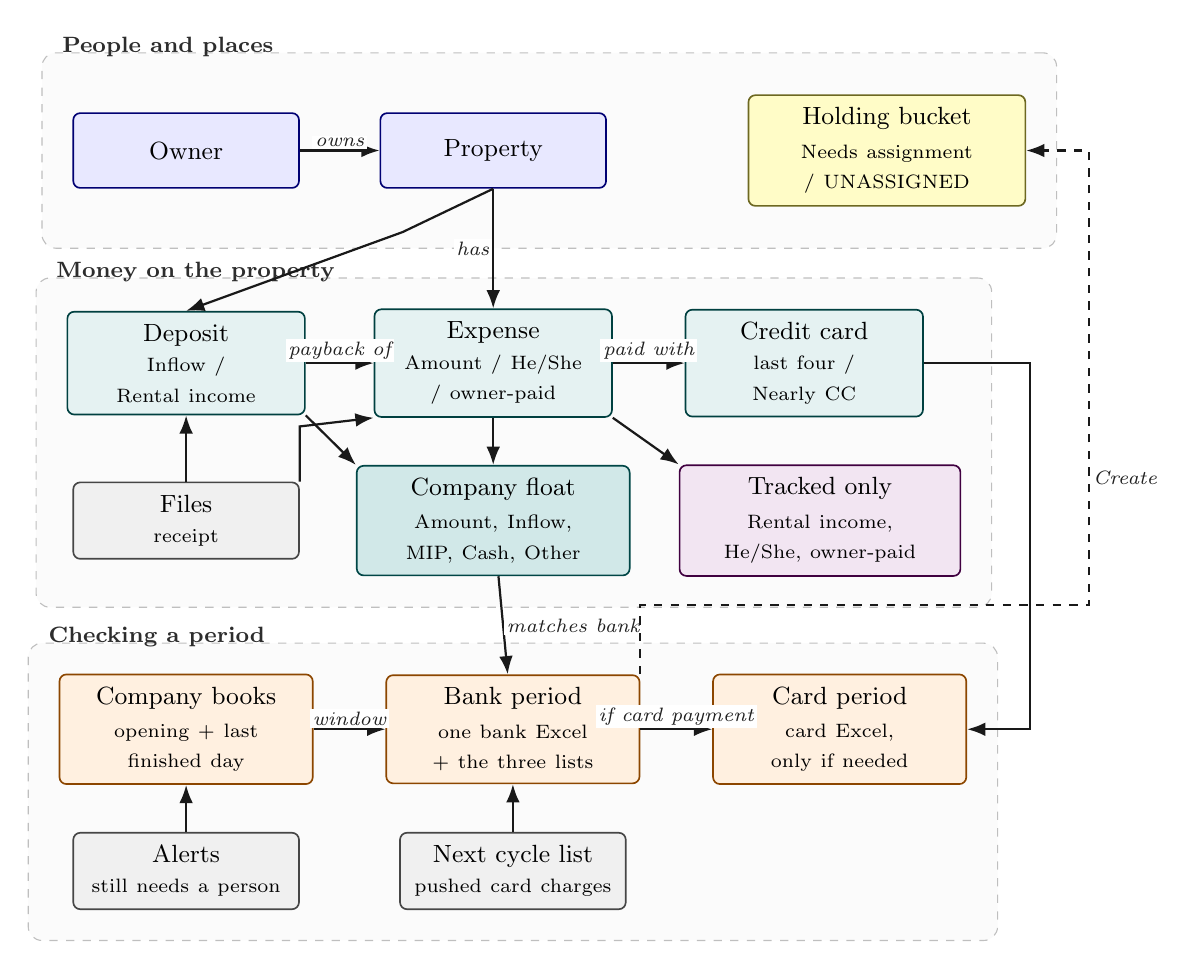
\begin{tikzpicture}[
  font=\small,
  >=Latex,
  box/.style={
    draw, rounded corners=2.5pt, align=center, inner sep=4.5pt,
    minimum height=0.95cm, line width=0.6pt
  },
  who/.style={box, fill=blue!9, draw=blue!45!black, text width=2.55cm},
  money/.style={box, fill=teal!10, draw=teal!50!black, text width=2.7cm},
  cfloat/.style={box, fill=teal!18, draw=teal!55!black, text width=3.15cm},
  track/.style={box, fill=violet!10, draw=violet!50!black, text width=3.25cm},
  chk/.style={box, fill=orange!12, draw=orange!55!black, text width=2.9cm},
  help/.style={box, fill=gray!12, draw=gray!55!black, text width=2.55cm},
  hold/.style={box, fill=yellow!22, draw=olive!70!black, text width=3.2cm},
  cluster/.style={
    draw=gray!50, dashed, rounded corners=5pt, inner sep=10pt,
    fill=gray!3
  },
  arr/.style={->, thick, draw=gray!20!black},
  lab/.style={font=\scriptsize\itshape, text=gray!25!black, align=center, fill=white, inner sep=1pt},
  bandlab/.style={font=\footnotesize\bfseries, text=gray!35!black}
]
  \node[who] (owner) at (0,0) {Owner};
  \node[who] (prop) at (3.9,0) {Property};
  \node[hold] (hold) at (8.9,0) {Holding bucket\\[1pt]
    {\scriptsize Needs assignment / UNASSIGNED}};

  \node[money] (dep) at (0,-2.7) {Deposit\\{\scriptsize Inflow / Rental income}};
  \node[money] (exp) at (3.9,-2.7) {Expense\\{\scriptsize Amount / He/She / owner-paid}};
  \node[money] (card) at (7.85,-2.7) {Credit card\\{\scriptsize last four / Nearly CC}};
  \node[help] (files) at (0,-4.7) {Files\\{\scriptsize receipt}};
  \node[cfloat] (cfloat) at (3.9,-4.7) {Company float\\[1pt]
    {\scriptsize Amount, Inflow, MIP, Cash, Other}};
  \node[track] (tracked) at (8.05,-4.7) {Tracked only\\[1pt]
    {\scriptsize Rental income, He/She, owner-paid}};

  \node[chk] (books) at (0,-7.35) {Company books\\[1pt]
    {\scriptsize opening + last finished day}};
  \node[chk] (bankp) at (4.15,-7.35) {Bank period\\[1pt]
    {\scriptsize one bank Excel + the three lists}};
  \node[chk] (cardp) at (8.3,-7.35) {Card period\\[1pt]
    {\scriptsize card Excel, only if needed}};
  \node[help] (alerts) at (0,-9.15) {Alerts\\{\scriptsize still needs a person}};
  \node[help] (nextc) at (4.15,-9.15) {Next cycle list\\{\scriptsize pushed card charges}};

  \begin{scope}[on background layer]
    \node[cluster, fit=(owner)(prop)(hold), inner ysep=15pt, inner xsep=11pt]
      (whoC) {};
    \node[cluster, fit=(dep)(exp)(card)(files)(cfloat)(tracked), inner sep=11pt]
      (moneyC) {};
    \node[cluster, fit=(books)(bankp)(cardp)(alerts)(nextc), inner sep=11pt]
      (checkC) {};
  \end{scope}

  \node[bandlab, above=2pt of whoC.north west, anchor=west, xshift=4pt]
    {People and places};
  \node[bandlab, above=2pt of moneyC.north west, anchor=west, xshift=4pt]
    {Money on the property};
  \node[bandlab, above=2pt of checkC.north west, anchor=west, xshift=4pt]
    {Checking a period};

  \draw[arr] (owner) -- node[lab, above] {owns} (prop);
  \draw[arr] (prop.south) -- node[lab, left] {has} (exp.north);
  \draw[arr] (prop.south) -- ++(-1.15,-0.55) -- (dep.north);
  \draw[arr] (exp) -- node[lab, above] {paid with} (card);
  \draw[arr] (dep) -- node[lab, above] {payback of} (exp);
  \draw[arr] (files) -- (dep);
  \draw[arr] (files.north east) -- ++(0,0.7) -- (exp.south west);

  \draw[arr] (dep.south east) -- (cfloat.north west);
  \draw[arr] (exp) -- (cfloat);
  \draw[arr] (exp.south east) -- (tracked.north west);

  \draw[arr] (books) -- node[lab, above] {window} (bankp);
  \draw[arr] (bankp) -- node[lab, above] {if card payment} (cardp);
  \draw[arr] (cfloat) -- node[lab, right] {matches bank} (bankp);
  \draw[arr] (card.east) -- ++(1.35,0) |- (cardp.east);
  \draw[arr, dashed] (bankp.north east) -- ++(0,0.88) -- ++(5.7,0) |-
    node[lab, pos=0.14, right] {Create} (hold.east);
  \draw[arr] (nextc) -- (bankp);
  \draw[arr] (alerts) -- (books);
\end{tikzpicture}
\caption{Data --- who owns the property, the money columns from the
Management expenses sheet, and the period check that stamps those same
rows against the bank.}
\label{fig:data}
\end{figure}

How to read it:
\begin{itemize}[itemsep=0.12em, topsep=0.3em]
  \item \textbf{Owner $\rightarrow$ property $\rightarrow$ expense / deposit}
        is the ledger. Dashboard, Owners, Properties, Reports, and AI all
        \emph{read} this. They do not hold a separate copy of the money.
  \item The money names are the columns on the \textbf{Management expenses
        sheet} (one tab per property). That workbook is the ground we test
        against.
  \item \textbf{Company float} (Amount, Inflow, plus MIP / Cash / Other when
        those columns exist) is what Verification matches to the company
        bank account.
  \item \textbf{Tracked only} (Rental income, He/She paid, owner-paid) stays
        in the ledger and in reports. It is not matched to the company bank.
  \item \textbf{Credit card} (last four, Nearly CC / Method): shop charges
        are still expenses on a property. They are checked on the card Excel,
        not as separate bank lines.
  \item \textbf{Bank period} is one bank Excel and the decisions on its lines,
        not a second ledger. \textbf{Card period} exists only if that Excel
        contains a card payment.
  \item \textbf{Holding} is Create-from-the-bank until a real owner and
        property are named. \textbf{Files} are the receipt column.
        \textbf{Next cycle} is postponed card charges (same rows).
        \textbf{Alerts} are reminders, not money.
\end{itemize}

\inapp{A payback is its own deposit, optionally linked to the original
expense --- it does not rewrite the expense. Company books (opening balance
and ``checked through'') live in Bank settings.}

% ---- PROCESS ----------------------------------------------------------------
\subsection{Process --- how work moves}
\label{sec:process-picture}

This is the same spine as later sections, drawn as a path.
Blue is the weekly loop. Teal / orange / yellow are the three Excel cases.
Green is a finished period.
Step 6 is the gate already described later: lists handled, holding assigned,
totals match.

\begin{figure}[H]
\centering
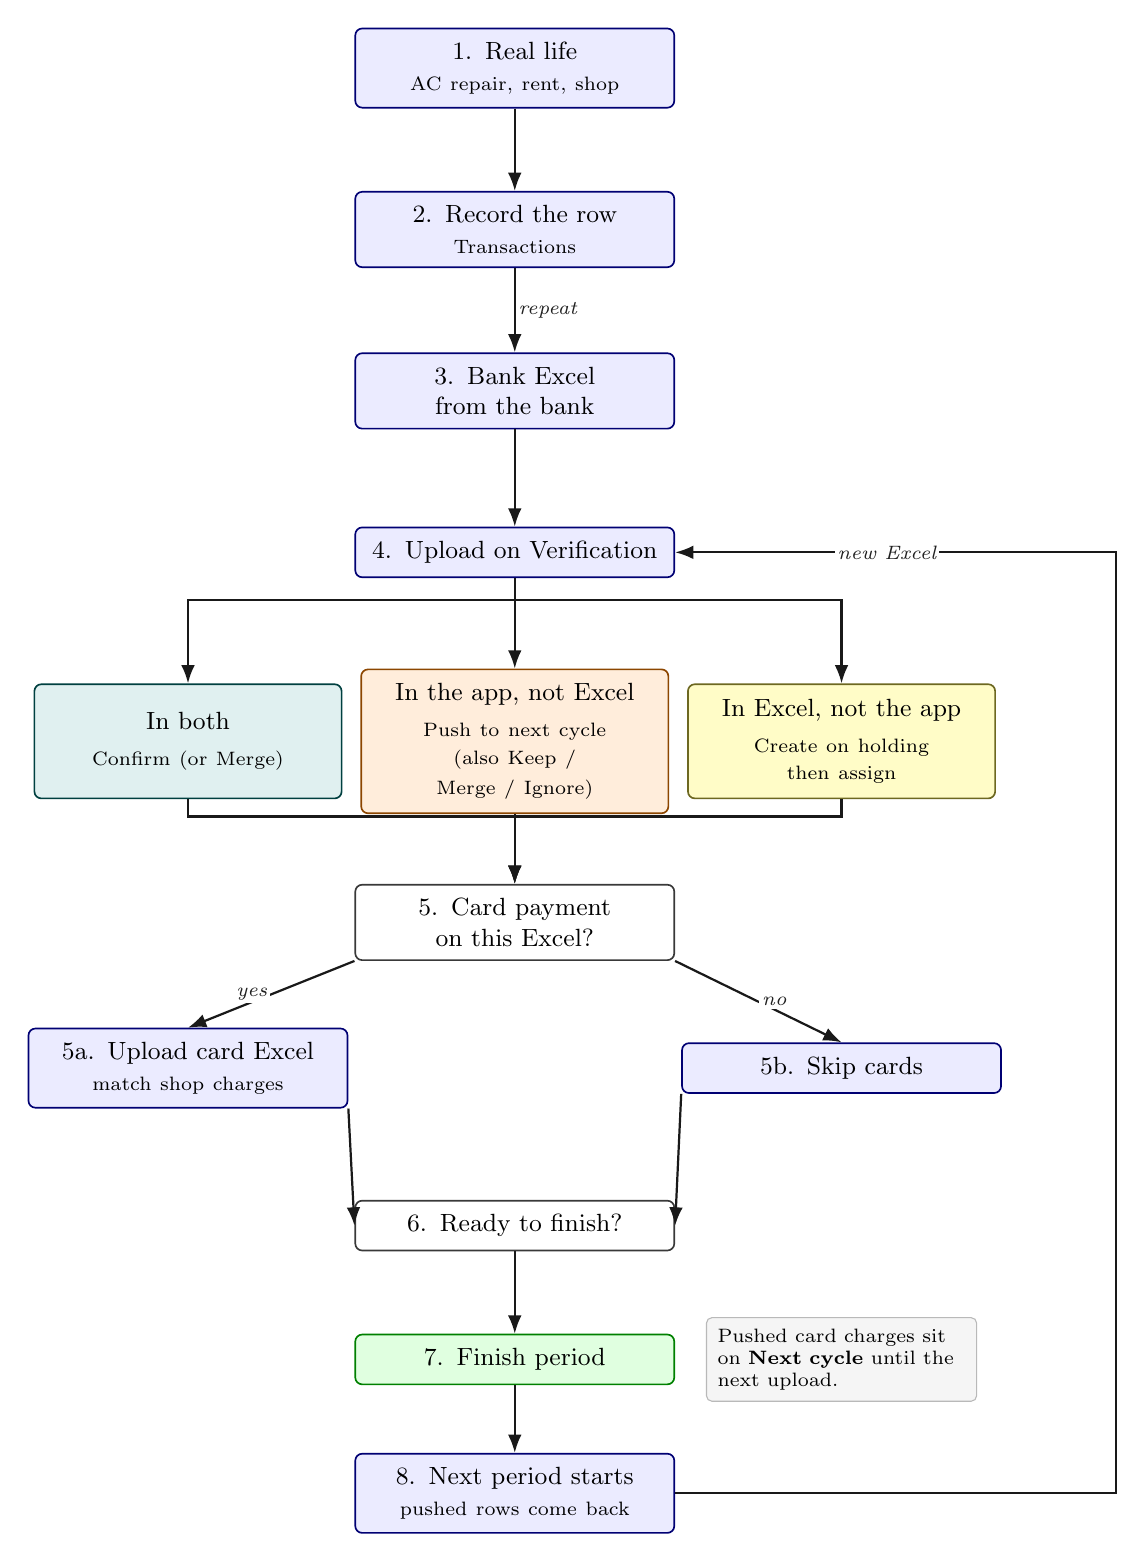
\begin{tikzpicture}[
  font=\small,
  >=Latex,
  wkbox/.style={
    draw, rounded corners=2.5pt, align=center, inner sep=5pt,
    text width=3.7cm, line width=0.6pt,
    fill=blue!8, draw=blue!45!black
  },
  fork/.style={
    draw, rounded corners=2.5pt, align=center, inner sep=5pt,
    text width=3.55cm, line width=0.6pt, minimum height=1.45cm
  },
  both/.style={fork, fill=teal!12, draw=teal!50!black},
  apponly/.style={fork, fill=orange!14, draw=orange!55!black},
  xlonly/.style={fork, fill=yellow!22, draw=olive!70!black},
  gate/.style={
    draw, rounded corners=2.5pt, align=center, inner sep=5pt,
    text width=3.7cm, line width=0.6pt,
    fill=white, draw=gray!45!black
  },
  done/.style={
    draw, rounded corners=2.5pt, align=center, inner sep=5pt,
    text width=3.7cm, line width=0.6pt,
    fill=green!12, draw=green!50!black
  },
  note/.style={
    draw=gray!55, rounded corners=2pt, align=left, inner sep=4pt,
    font=\scriptsize, text width=3.15cm, fill=gray!8
  },
  arr/.style={->, thick, draw=gray!20!black},
  lab/.style={font=\scriptsize\itshape, text=gray!25!black, fill=white, inner sep=1pt}
]
  \node[wkbox] (life) at (0,0) {1. Real life\\{\scriptsize AC repair, rent, shop}};
  \node[wkbox] (rec) at (0,-2.05) {2. Record the row\\{\scriptsize Transactions}};
  \node[wkbox] (xl) at (0,-4.1) {3. Bank Excel from the bank};
  \node[wkbox] (up) at (0,-6.15) {4. Upload on Verification};

  \draw[arr] (life) -- (rec);
  \draw[arr] (rec) -- node[lab, right] {repeat} (xl);
  \draw[arr] (xl) -- (up);

  \node[both] (c1) at (-4.15,-8.55) {In both\\[2pt]
    {\scriptsize Confirm (or Merge)}};
  \node[apponly] (c2) at (0,-8.55) {In the app, not Excel\\[2pt]
    {\scriptsize Push to next cycle}\\[-1pt]
    {\scriptsize (also Keep / Merge / Ignore)}};
  \node[xlonly] (c3) at (4.15,-8.55) {In Excel, not the app\\[2pt]
    {\scriptsize Create on holding}\\[-1pt]
    {\scriptsize then assign}};

  \draw[arr] (up.south) -- ++(0,-0.28) -| (c1.north);
  \draw[arr] (up) -- (c2);
  \draw[arr] (up.south) -- ++(0,-0.28) -| (c3.north);

  \node[gate] (ccq) at (0,-10.85) {5. Card payment on this Excel?};
  \node[wkbox] (ccyes) at (-4.15,-12.7) {5a. Upload card Excel\\{\scriptsize match shop charges}};
  \node[wkbox] (ccno) at (4.15,-12.7) {5b. Skip cards};

  \draw[arr] (c1.south) -- ++(0,-0.22) -| (ccq.north);
  \draw[arr] (c2) -- (ccq);
  \draw[arr] (c3.south) -- ++(0,-0.22) -| (ccq.north);
  \draw[arr] (ccq.south west) -- node[lab, left] {yes} (ccyes.north);
  \draw[arr] (ccq.south east) -- node[lab, right] {no} (ccno.north);

  \node[gate] (finq) at (0,-14.7) {6. Ready to finish?};
  \node[done] (fin) at (0,-16.4) {7. Finish period};
  \node[wkbox] (next) at (0,-18.1) {8. Next period starts\\{\scriptsize pushed rows come back}};

  \draw[arr] (ccyes.south east) -- (finq.west);
  \draw[arr] (ccno.south west) -- (finq.east);
  \draw[arr] (finq) -- (fin);
  \draw[arr] (fin) -- (next);
  \draw[arr] (next.east) -- ++(5.6,0) |-
    node[lab, pos=0.82, right] {new Excel} (up.east);

  \node[note] (nnote) at (4.15,-16.4) {Pushed card charges sit on
    \textbf{Next cycle} until the next upload.};
\end{tikzpicture}
\caption{Process --- record what happened, prove it against the bank Excel,
handle the three cases, check cards only when the bank paid the card
company, then finish and start the next period.}
\end{figure}

Around that loop, the other pages do not add a second workflow:

\begin{center}
\begin{tabular}{@{}p{0.34\textwidth}p{0.58\textwidth}@{}}
\toprule
\textbf{Page} & \textbf{Role in the process} \\
\midrule
Dashboard, Properties, Owners, Reports, AI Query
  & Read the same ledger. They do not change how a period is proved. \\
\addlinespace
Alerts
  & A work queue: unassigned rows, unmatched lines, missing deposit, low balance.
    Deep-links into Verification or Transactions. \\
\addlinespace
Credit cards
  & The card register (last four digits). Used when recording ``paid with card''
    and when a card Excel is uploaded. \\
\addlinespace
Next cycle
  & The waiting list of postponed card charges (step 8 coming back into step 4). \\
\addlinespace
Data import, Bank settings, Alert rules
  & Admin: load history, set opening / checked-through, set low-balance rules.
    Not the weekly check. \\
\bottomrule
\end{tabular}
\end{center}

\discuss{The picture shows all four actions when the app has a row the Excel
does not (Push, Keep, Merge, Ignore). If the meeting decides postpone is the
only allowed action, this figure is the first thing to edit.}

% -----------------------------------------------------------------------------
\section{Recording a real-life transaction}

\subsection{Where}

\textbf{Transactions} is the ledger.
It is the page used every week, not only at month-end.

From here she can:
\begin{itemize}
  \item add one \textbf{expense} (money out --- the air-conditioner bill);
  \item add one \textbf{deposit} (money in --- a transfer, a payback);
  \item attach files (receipt, invoice, photo);
  \item import a file (receipt PDF, generic Excel, or a statement);
  \item filter, edit, delete, and export CSV.
\end{itemize}

\subsection{What must be filled in}

For both an expense and a deposit the app requires:
\begin{itemize}
  \item an \textbf{owner},
  \item a \textbf{property},
  \item a \textbf{date},
  \item an \textbf{amount} greater than zero.
\end{itemize}

If those are missing, the row is not saved.

\subsection{How it was paid}

On an expense, \textbf{Paid with} says how the money left:
company account, cash, credit card (then the last four digits of the card),
and similar methods.

On a deposit, the matching idea is \textbf{Received with}.
A deposit can also be marked \textbf{Rental income} or \textbf{Payback}
(a refund that stays its own row, optionally linked to the original expense).

\inapp{Credit-card expenses need a card on the Credit cards page first.
If none exist, the form says to add a card there before choosing one.}

\subsection{What this row is, until the bank is checked}

A row typed by hand already has a real owner and property.
Until a bank (or card) statement confirms it, the app treats it as
\textbf{not yet verified} against the bank.

That is different from a row the bank invented during verification
(see~\S\ref{sec:excel-not-app}).

\subsection{Money that is tracked but not ``company float''}

The violet box in Figure~\ref{fig:data}:
\textbf{Rental income}, \textbf{He/She paid}, and \textbf{owner-paid}.
They stay in the ledger and in reports.
They are not what Verification matches to the company bank account.

\discuss{Confirm with the client that rental, He/She, and owner-paid stay
out of the bank check, as they do today.}

% -----------------------------------------------------------------------------
\section{Checking a period against the bank}
\label{sec:verify}

\subsection{When}

When she has a bank Excel for the period --- typically after several
transactions are already in the app.

Page: \textbf{Verification}.

The top of the page shows:
\begin{itemize}
  \item \textbf{Bank balance} --- opening, or the closing of the last
        finished period;
  \item \textbf{Checked through} --- the last day already finished;
  \item \textbf{Still to check} --- rows still waiting.
\end{itemize}

She uploads the bank Excel under \textbf{Step 1 · Bank statement}.

If that file has already been fully checked, the app says she is
caught up --- there are no new bank lines.

\subsection{What the upload is asking}

For every movement on the Excel, and every company-float row in the app
for that window, the period must end in one of three places:

\begin{enumerate}
  \item it is in \textbf{both} the app and the Excel;
  \item it is in the \textbf{app but not} the Excel;
  \item it is in the \textbf{Excel but not} the app.
\end{enumerate}

The identity she is proving is:

\begin{center}
\textit{Opening balance $+$ money in the app for this period
$=$ closing balance on the statement.}
\end{center}

She cannot finish while that is off by more than one agora (ILS~0.01),
or while any list item is still open, or while a bank-created row is
still sitting on \textbf{Needs assignment}.

% -----------------------------------------------------------------------------
\section{Case 1 --- the transaction is in the app and in the Excel}

This is the happy path.

Example: the air-conditioner expense was typed last week.
The bank Excel shows the same amount leaving the account.

The app puts it under \textbf{Found on statement}.

What she does:
\begin{itemize}
  \item \textbf{Confirm} that one row, or
  \item \textbf{Confirm all found}.
\end{itemize}

After confirm, that row is bank-verified.
It counts in this period's totals.

If the amounts are close but not the same, she can \textbf{Merge}:
the bank date, amount, and reference (\emph{asmachta}) win, and the app
row is updated to match the bank.

% -----------------------------------------------------------------------------
\section{Case 2 --- the transaction is in the app, not in the Excel}
\label{sec:app-not-excel}

The ledger already knows about the money.
The bank file for \emph{this} period does not show it leaving (or arriving).

Typical reason: the work was done, the row was typed, but the bank has
not paid yet --- it will show on the \emph{next} statement.

\subsection{What we want}

Postpone it to the next period.
When the next bank Excel arrives, match it to the bank line.

\subsection{What the app does today}

Those rows appear under \textbf{In the app, not on the statement}
(and, for some card leftovers, under \textbf{Not for this period}).

Actions available:
\begin{description}[style=nextline, leftmargin=1.4em]
  \item[Push to next cycle]
        The intended postpone.
        The row waits.
        It is listed on \textbf{Next cycle}.
        When the next verification starts, it is shown again so it can be
        matched to the bank (Merge / Confirm) if the money has now left.
  \item[Keep in this period]
        She decides it belongs in \emph{this} cycle even though it is not
        on this Excel (for example a card charge that should count now).
  \item[Merge]
        It is actually the same as a bank line that did not auto-match
        (wrong date or wording). Bank values overwrite the app row.
  \item[Ignore]
        Leave it out of this check, with a reason.
\end{description}

\discuss{The original story only named postpone.
The app also offers Keep, Merge, and Ignore.
Decide with the client whether postpone should be the only action
for ``in the app, not on the Excel'', or whether Keep / Merge / Ignore
should stay.}

% -----------------------------------------------------------------------------
\section{Case 3 --- the transaction is in the Excel, not in the app}
\label{sec:excel-not-app}

The bank shows money that was never typed.

Typical reasons: someone paid from the account and forgot to record it;
or the row was never imported.

\subsection{What we want}

Create the missing transaction.
It must not pretend to be a finished, assigned row.
Owner and property start as a holding bucket.
Those rows must be given a real owner and property before the period
can finish.

\subsection{What the app does today}

Those bank lines appear under \textbf{On the statement, not in the app}.

Actions:
\begin{description}[style=nextline, leftmargin=1.4em]
  \item[Create]
        Makes the deposit or expense from the bank line.
        Owner is \textbf{Needs assignment}.
        Property is \textbf{UNASSIGNED}.
        The row is flagged for handling.
        An alert is raised until it is assigned.
  \item[Create payback]
        Same idea, for a bank credit that is a refund / partial return.
  \item[Merge]
        Link this bank line to an existing app row that is the same
        transaction (bank values win).
  \item[Ignore]
        Do not create it; give a reason.
\end{description}

After Create she uses \textbf{Edit} on that row:
pick the real owner and property, section, paid-with, notes, files.

\inapp{The holding names in the app are \textbf{Needs assignment}
(owner) and \textbf{UNASSIGNED} (property) --- not the phrase
``unverified transaction''.
A row she typed herself with a real property is simply unverified
until the bank confirms it.
A row the bank created is \emph{unassigned} until she names it.}

\discuss{If the client prefers the words ``unverified transaction''
on that holding owner/property, that is a label change we can make.
The rule itself already matches: create from the bank, then assign
before the period can end.}

% -----------------------------------------------------------------------------
\section{Finishing the period}

\textbf{Finish period} stays off until all of the following are true:

\begin{enumerate}
  \item every bank line is confirmed, created, merged, or ignored;
  \item every leftover app row is merged, postponed, kept, or ignored;
  \item no bank-created row is still on Needs assignment / UNASSIGNED;
  \item opening $+$ app net $=$ closing, within ILS~0.01.
\end{enumerate}

If the totals are off, the app says the period is off by ILS~X and asks
her to create a transaction for that amount.

Finished periods stay on Verification as history
(\textbf{Finished periods}), with a badge for totals match or totals off.
They are view-only.

\discuss{Finish-only-when-balanced is strict on purpose.
Confirm she wants no ``finish anyway''.}

% -----------------------------------------------------------------------------
\section{Credit cards}
\label{sec:cards}

Cards sit \emph{under} verification, not as a separate monthly ritual.

\subsection{When cards are required}

If the bank Excel contains a card payment (the Mastercard / card-settlement
line), Step~2 \textbf{Credit card} appears:
``Your bank statement includes a card payment --- upload that card
statement next.''

She uploads each card's Excel, confirms matches, creates missing card
charges, or postpones charges that are not on this card file.

\subsection{When cards are ignored}

If the bank Excel has \emph{no} card payment, the app says:
``No card payment on this statement --- no card check needed.''
She does not upload card files for that period.

\subsection{The two layers}

\begin{enumerate}
  \item \textbf{Card statement} --- each shop charge (the air-conditioner
        paid by card) is matched to the card Excel.
  \item \textbf{Bank statement} --- the lump sum the bank paid the card
        company is the settlement line. Confirm it once the card side
        is in order. Individual shop charges are not re-matched one-by-one
        to the company bank account, unless they were postponed and the
        money later leaves the bank as its own debit.
\end{enumerate}

\subsection{Cards as a list}

\textbf{Credit cards} is a small register: last four digits, optional name,
active / inactive, view that card's transactions.
Cards are also created automatically when a new card statement is uploaded.

\subsection{Next cycle}

\textbf{Next cycle} lists card charges that were pushed forward
(``after this date'').
They reappear at the top of Verification when the next statement is opened,
so they can be kept, pushed again, or matched to the bank.

\discuss{Confirm the rule: card step only when the bank file shows a card
payment; otherwise skip cards for that period. That is how the app works
now.}

% -----------------------------------------------------------------------------
\section{A picture of one period}

\begin{center}
\begin{tabular}{@{}p{0.28\textwidth}p{0.32\textwidth}p{0.32\textwidth}@{}}
\toprule
\textbf{In real life} & \textbf{In the app} & \textbf{On the bank Excel} \\
\midrule
AC repaired, paid from the company account &
Expense typed on Transactions &
Same debit $\rightarrow$ Found $\rightarrow$ Confirm \\
\addlinespace
AC repaired, typed, bank has not paid yet &
Expense already in the ledger &
Missing $\rightarrow$ Push to next cycle \\
\addlinespace
Someone paid from the account, never typed &
Nothing yet &
Create $\rightarrow$ Needs assignment $\rightarrow$ assign before finish \\
\addlinespace
Shop charge on the company card &
Expense paid with card &
Card Excel in Step~2; bank only shows the card payment lump \\
\bottomrule
\end{tabular}
\end{center}

% -----------------------------------------------------------------------------
\section{The rest of the app}

These pages are not the main loop.
They make the loop usable.

\subsection{Dashboard}

The overview for a month, quarter, or year:
deposits, expenses, net, open alerts, property health, recent activity.
Jumps into Transactions or Alerts.

\subsection{Properties}

The property list: owner, incoming, outgoing, balance, active / inactive.
Incoming here is company float (not rental).
Outgoing excludes He/She and owner-paid.
Opens that property's transactions.

\subsection{Owners}

The same idea rolled up by owner.
Inactive means every linked property is inactive.

\subsection{Alerts}

Things that still need a person:
\begin{itemize}
  \item missing expected deposit;
  \item incomplete import (missing date or amount);
  \item needs assignment (UNASSIGNED rows);
  \item unmatched bank / unmatched app / gap, while a period is open;
  \item unmatched card lines;
  \item low balance (threshold set by an admin).
\end{itemize}

Reconcile alerts deep-link to Verification.
Assignment alerts can open Transactions or Verification.

\subsection{Reports}

Simple totals by owner or by property.
Links back to Owners / Properties.

\subsection{AI Query}

Ask in plain language (``electricity this quarter'').
Opens matching rows in Transactions or exports Excel.

\subsection{Data import} (admin)

Load the client's workbooks (client list + Management expenses sheet) into the
database. Can reset the database first.
This is how a full history is brought in --- not the weekly bank check.

\subsection{Bank settings} (admin)

Opening balance, the date the books start, ``bank verified through'',
and how tight the gap may be.
A cutover can mark everything up to a date as already verified.

\subsection{Alert rules} (admin)

Low-balance threshold, globally or per property.

\subsection{Feedback}

Any page: send a problem or an idea by email.

% -----------------------------------------------------------------------------
\section{Words we use}

\renewcommand{\arraystretch}{1.15}
\begin{tabularx}{\textwidth}{@{}>{\raggedright\arraybackslash}p{0.34\textwidth}>{\raggedright\arraybackslash}X@{}}
\toprule
\textbf{Everyday / client wording} & \textbf{Label in the app today} \\
\midrule
The ledger & Transactions \\
Check the period against the bank & Verification \\
In both app and Excel & Found on statement \\
In the app, not on this Excel & In the app, not on the statement \\
On the Excel, not in the app & On the statement, not in the app \\
Postpone until the bank pays & Push to next cycle \\
Count it in this period anyway & Keep in this period \\
Same transaction, fix the app from the bank & Merge \\
Bank created a row we have not named & Needs assignment / UNASSIGNED \\
Typed row, bank has not confirmed it yet & Unverified \\
Card shop charge waiting for a later file & Next cycle / Credit card postponed \\
Company running total & Inflow / Expenses / Balance (excludes rental and He/She) \\
\bottomrule
\end{tabularx}

% -----------------------------------------------------------------------------
\section{Suggested agenda with the client}

Walk these in order, with the live app open:

\begin{enumerate}
  \item Tell the air-conditioner story once, without the screen.
  \item Add that expense on Transactions (owner, property, date, amount,
        paid with).
  \item Open Verification and upload a bank Excel.
  \item Point at the three lists. Do one Confirm, one Push, one Create.
  \item Assign the created row off Needs assignment.
  \item Show Finish blocked while the gap is off, then matching totals.
  \item Show a statement \emph{with} a card payment (Step~2 appears) and
        one \emph{without} (``no card check needed'').
  \item Open Next cycle and Alerts so she sees leftovers and assignment
        warnings.
\end{enumerate}

Then decide, in writing:

\begin{itemize}
  \item Is postpone the only action when the app has a row the Excel does
        not? (Today: Push, Keep, Merge, Ignore.)
  \item Are the holding names ``Needs assignment / UNASSIGNED'' acceptable,
        or should they read ``unverified transaction''?
  \item Must every period close at ILS~0.00, with no finish-anyway?
  \item Do rental, He/She, and owner-paid stay off the bank check?
  \item Is the card step only when the bank file shows a card payment?
\end{itemize}

\vspace{1.2em}
\noindent\textit{This draft follows the app as it behaves in September 2026.
Edit the yellow boxes after the meeting; they are the change list.}

\end{document}
